% See http://tex.stackexchange.com/questions/168169/options-for-supplementary-materials-in-preprint-version-revtex-arxiv

\pagebreak
\begin{center}
\textbf{\large Supplemental Materials}
\end{center}

\setcounter{equation}{0}
\setcounter{figure}{0}
\setcounter{table}{0}
\makeatletter
\renewcommand{\theequation}{S\arabic{equation}}
\renewcommand{\thefigure}{S\arabic{figure}}

\begin{center}
    \begin{tabular}{ | l | p{8cm} |}
    \hline
    Data File & Description \\ \hline
    \texttt{all\_signatures.csv} & Mutational signatures used for deconvolution. Includes COSMIC curated signatures and the signatures extracted from the Meier et al.~\cite{Meier_2014} and Szikriszt et al.~\cite{Szikriszt_2016} studies. \\ \hline
    % \texttt{bayesian\_model\_fit\_coefficients.csv} & MCMC samples for the Bayesian model \\ \hline
    \texttt{deconstructsigs\_output.cleaned.csv} & deconstructSigs results \\ \hline
    \texttt{hla\_types.csv} & HLA types for AOCS patients inferred from DNA and RNA sequencing \\ \hline
    \texttt{annotated\_mutations.with\_mhc\_binders.csv.bz2} & All mutation calls \\ \hline
    \texttt{sources.extended.with\_signature\_counts.csv} & Metadata for each AOCS tissue sample \\ \hline
    \texttt{treatments\_matrix.csv} & Clinical treatment data for AOCS patients \\ \hline
    \end{tabular}
\end{center}


\section*{Supplemental Figures}

\FloatBarrier

\begin{figure}
\centering
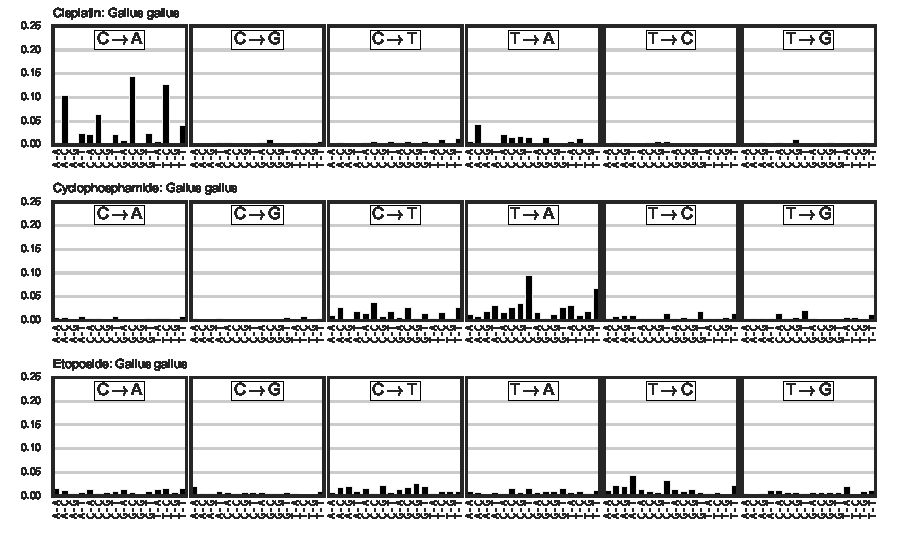
\includegraphics[scale=1.0]{figures/extracted_signatures_chicken.pdf}
\caption{Mutational signatures extracted from Szikriszt et al.~\cite{Szikriszt_2016}}
\label{fig:supp_extracted_signatures_chicken}
\end{figure}

\begin{figure}
\centering
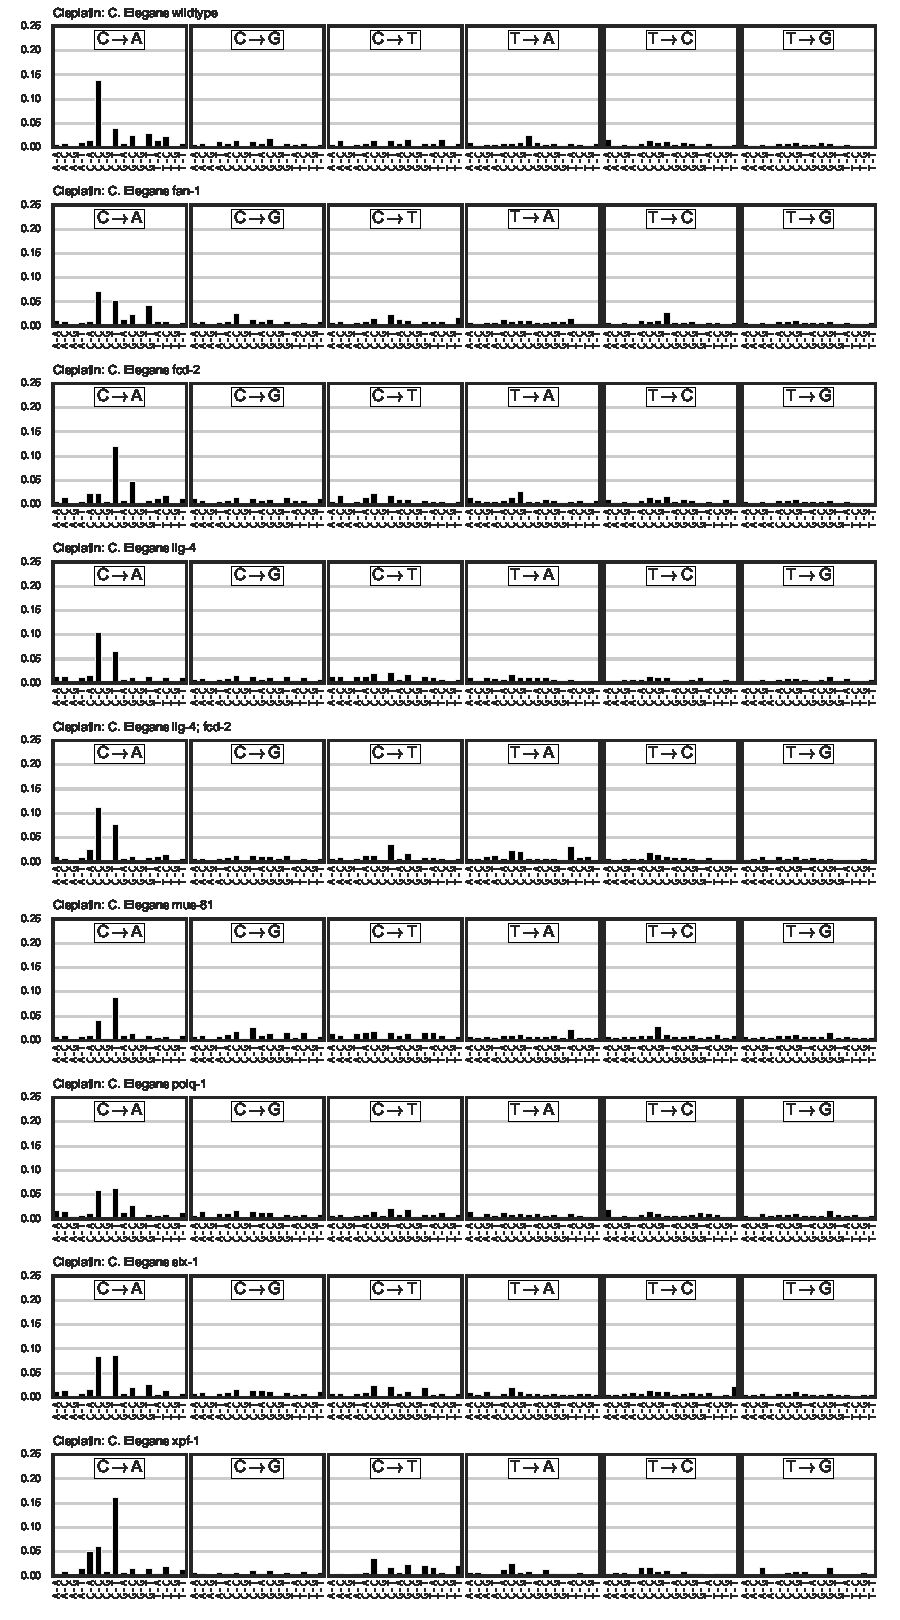
\includegraphics[scale=1.0]{figures/extracted_signatures_worm.pdf}
\caption{Mutational signature extracted from Meier et al.~\cite{Meier_2014}}
\label{fig:supp_extracted_signatures_worm}
\end{figure}

\begin{figure}
\centering
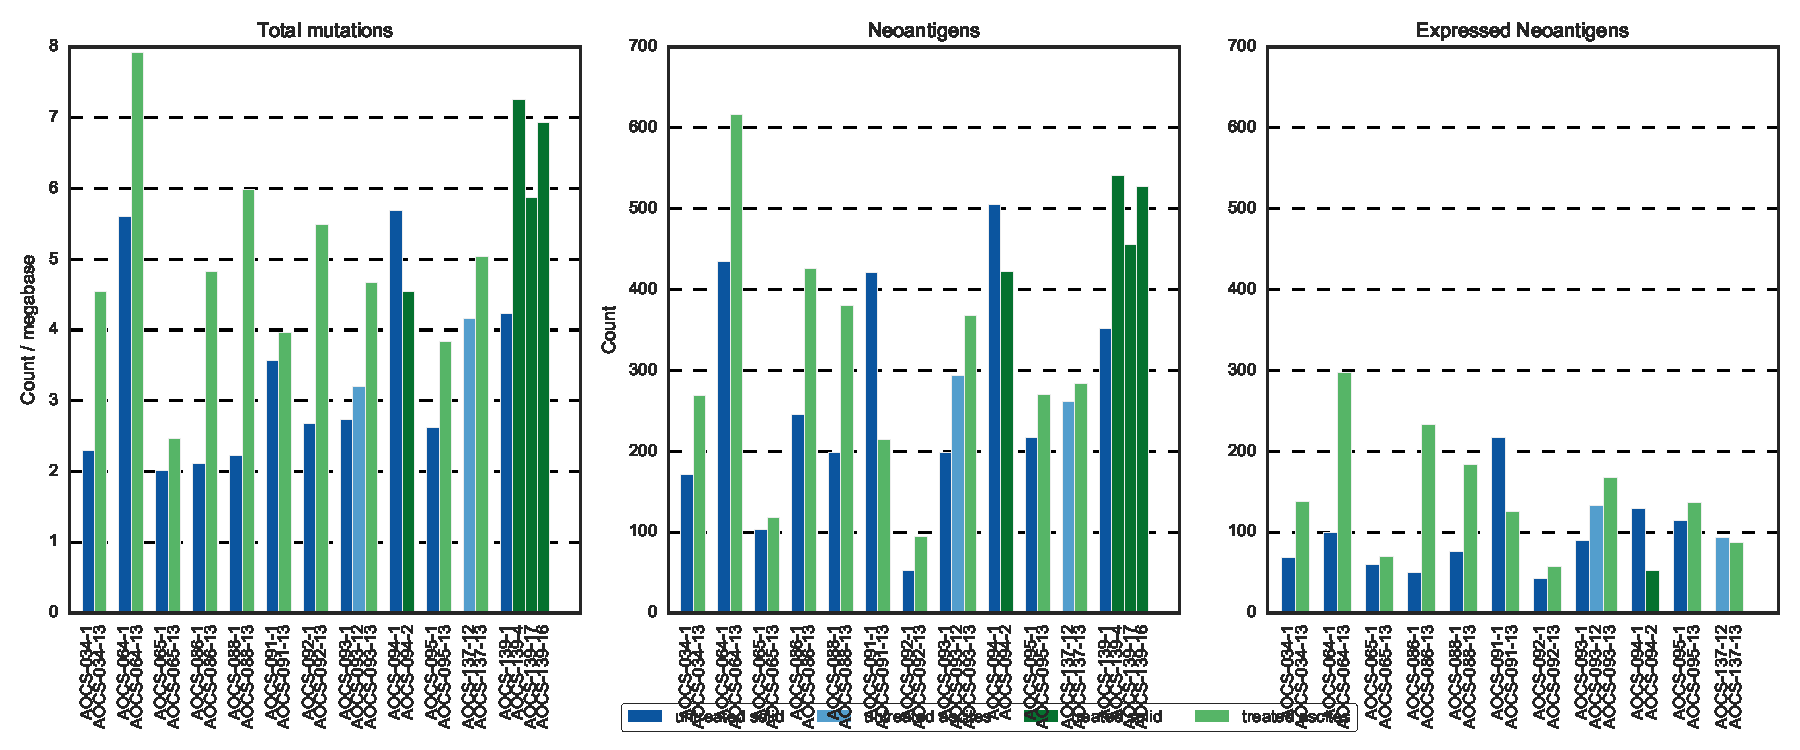
\includegraphics[scale=1.0]{figures/paired_counts.pdf}
\caption{Mutations, neoantigens, and expressed neoantigens for the patients with paired pre-/post-chemotherapy samples.}
\label{fig:supp_paired}
\end{figure}

\begin{figure}
\centering
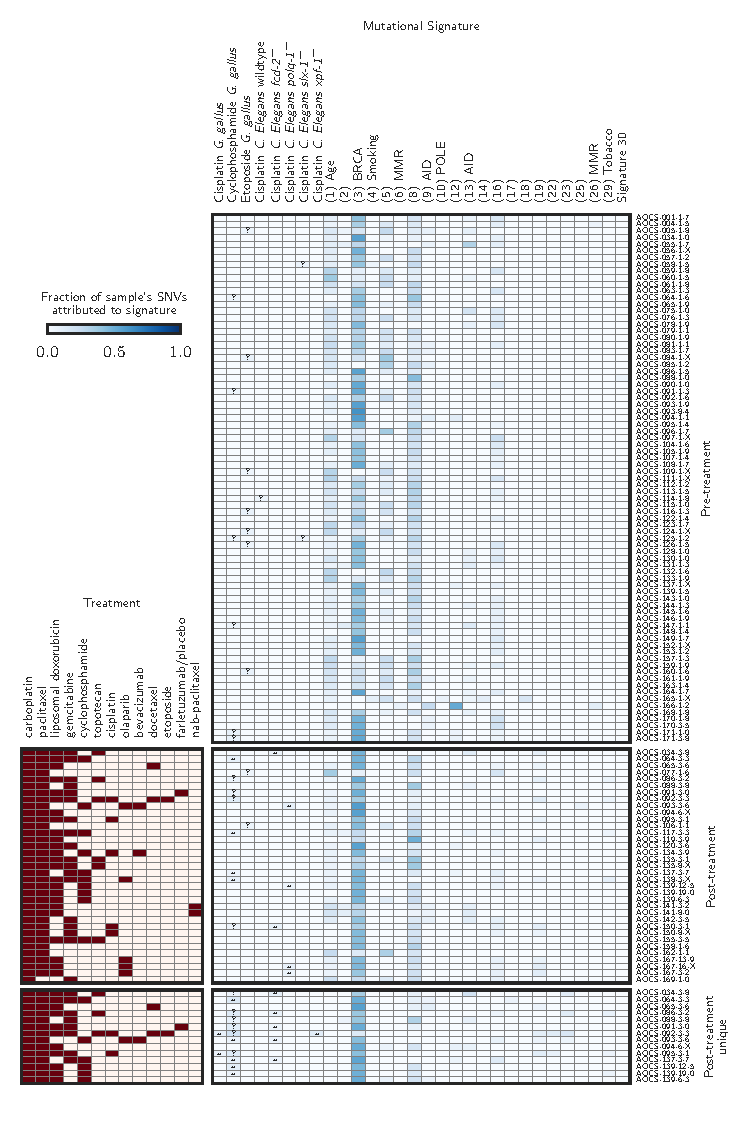
\includegraphics[scale=1.0]{figures/supplementary_signatures.pdf}
\caption{\textbf{Mutational signature deconvolutions for all samples.} The symbols are as in main text Figure~\ref{fig:signatures}.}
\label{fig:supp_signatures}
\end{figure}

\begin{figure}
\centering
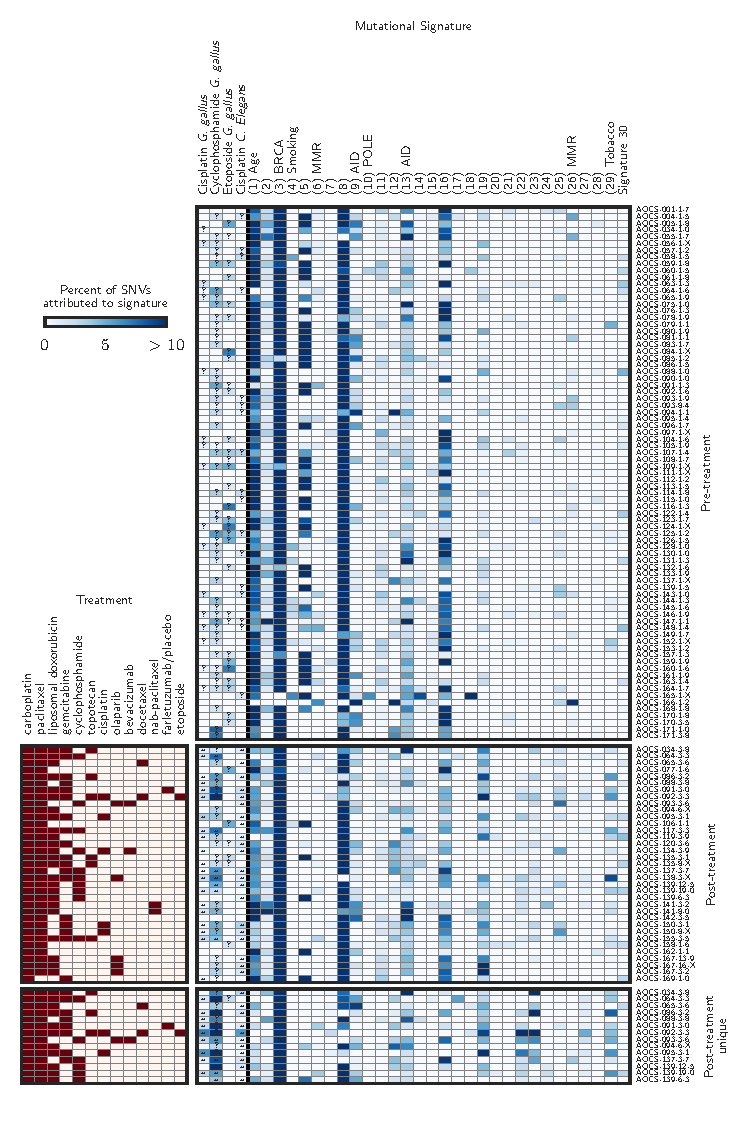
\includegraphics[scale=1.0]{figures/supplementary_signatures_no_cutoff.pdf}
\caption{\textbf{Mutational signature deconvolutions for all samples, without any minimum threshold.} Signatures accounting for less than the 6\% recommended threshold are included. The symbols are as in main text Figure~\ref{fig:signatures}.}
\label{fig:supplementary_signatures_no_cutoff.pdf}
\end{figure}

\FloatBarrier
